%%%%%%%%%%%%%%%%%%%%%%%%%%%%%%%%%%%%%%%%%
% Short Sectioned Assignment
% LaTeX Template
% Version 1.0 (5/5/12)
%
% This template has been downloaded from:
% http://www.LaTeXTemplates.com
%
% Original author:
% Frits Wenneker (http://www.howtotex.com)
%
% License:
% CC BY-NC-SA 3.0 (http://creativecommons.org/licenses/by-nc-sa/3.0/)
%
%%%%%%%%%%%%%%%%%%%%%%%%%%%%%%%%%%%%%%%%%

%----------------------------------------------------------------------------------------
%	PACKAGES AND OTHER DOCUMENT CONFIGURATIONS
%----------------------------------------------------------------------------------------

\documentclass[paper=a4, fontsize=11pt]{scrartcl} % A4 paper and 11pt font size

\usepackage[T1]{fontenc} % Use 8-bit encoding that has 256 glyphs
\usepackage{fourier} % Use the Adobe Utopia font for the document - comment this line to return to the LaTeX default
\usepackage[english]{babel} % English language/hyphenation
\usepackage{amsmath,amsfonts,amsthm} % Math packages

\usepackage{graphicx}
\graphicspath{ {images_12_8_16/} }

\usepackage{lipsum} % Used for inserting dummy 'Lorem ipsum' text into the template
\usepackage{url}

\usepackage{sectsty} % Allows customizing section commands
\allsectionsfont{\centering \normalfont\scshape} % Make all sections centered, the default font and small caps

\usepackage{fancyhdr} % Custom headers and footers
\pagestyle{fancyplain} % Makes all pages in the document conform to the custom headers and footers
\fancyhead{} % No page header - if you want one, create it in the same way as the footers below
\fancyfoot[L]{} % Empty left footer
\fancyfoot[C]{} % Empty center footer
\fancyfoot[R]{\thepage} % Page numbering for right footer
\renewcommand{\headrulewidth}{0pt} % Remove header underlines
\renewcommand{\footrulewidth}{0pt} % Remove footer underlines
\setlength{\headheight}{13.6pt} % Customize the height of the header

\numberwithin{equation}{section} % Number equations within sections (i.e. 1.1, 1.2, 2.1, 2.2 instead of 1, 2, 3, 4)
\numberwithin{figure}{section} % Number figures within sections (i.e. 1.1, 1.2, 2.1, 2.2 instead of 1, 2, 3, 4)
\numberwithin{table}{section} % Number tables within sections (i.e. 1.1, 1.2, 2.1, 2.2 instead of 1, 2, 3, 4)

\setlength\parindent{0pt} % Removes all indentation from paragraphs - comment this line for an assignment with lots of text

%----------------------------------------------------------------------------------------
%	TITLE SECTION
%----------------------------------------------------------------------------------------

\newcommand{\horrule}[1]{\rule{\linewidth}{#1}} % Create horizontal rule command with 1 argument of height

\title{	
\normalfont \normalsize 
\textsc{Deep Learning for Computer Graphics, Fall 2016} \\ [25pt] % Your university, school and/or department name(s)
\horrule{0.5pt} \\[0.4cm] % Thin top horizontal rule
\huge Deep Reinforcement Learning for Atari (Ms. Pac-Man) \\ % The assignment title
\horrule{2pt} \\[0.5cm] % Thick bottom horizontal rule
}

\author{Prabhat Rayapati (pr2sn), Zack Verham (zdv8rb)} % Your name

\date{\normalsize\today} % Today's date or a custom date

\begin{document}

\maketitle % Print the title

\section{Project Goal}

The goal of this project was to attempt to implement the deep reinforcement pipeline utilized in ``Playing Atari with Deep Reinforcement Learning"\footnote{\url{https://arxiv.org/pdf/1312.5602.pdf}}, proposed in 2013 by Mnih et. al., in order to teach a reinforcement-learning actor how to play Ms. Pac-Man on an Atari emulator. Ultimately, our purpose in undertaking this project was to learn both the technical details outlined in the paper, and the general process of implementing an agent which can play video games using deep learning techniques. 

\section{Group + Contributions}

Our project group consisted of Prabhat Rayapati (pr2sn), and Zack Verham (zdv8rb). While ultimately both group members were involved in all aspects of the project, especially when it came to understanding and implementing the underlying details of the learning agent, Prabhat focused on implementing many of the visualization tools used to understand the learning and decision-making process utilized by the agent, and Zack focused on interfacing the agent with the OpenAI Gym\footnote{\url{https://gym.openai.com/}} codebase. However, writing the actual code wasn't the primary hurdle for this project; rather, understanding the underlying algorithm took the most time, and our personal contributions on that front were equally split, since comprehension mostly came about through inter-group discussion and consistent team meetings.

\section{Achieved Milestones}

\begin{enumerate}
\item Connect a decision-making agent with an Atari emulator
\item Implement the essentials of the deep learning architecture proposed in the ``Atari Deep Learning" paper using Keras
\item Incorporate additional learning facilitators utilized in the ``Atari Deep Learning" paper (experience replay, decaying epsilon value, temporally stacked input frames, etc.)
\item Implement a baseline random decision-making agent, compare reward-per-game to validate that our learner improves over random
\end{enumerate}

\section{Challenges}

The biggest challenge for us was wrestling with the training time necessary for our deep reinforcement learning agents to learn effective policies. Some documents on deep reinforcement learning describe this process taking several days to complete\footnote{\url{http://karpathy.github.io/2016/05/31/rl/}}. This time investment made it challenging to (a) debug our implementation, since there were certain memory constraints which only appeared after thousands of episodes of training, and (b) to tune the setting of our hyperparameters. The memory bugs in particular constrained the number of episodes run in our final results. However, we believe that these challenges could be overcome quite easily if the time constraints of an end-of-semester project were removed.

\section{Results}

In our final training runs, our deep learning agent and random agent played 2099 and 699 games of Ms. Pac-Man, respectively. Our primary result is that, on average, our learning agent attains an increasing average reward-per-game over time, while a naive baseline agent which only makes random decisions generates a non-increasing average reward-per-game. The results from our random agent are illustrated in Figure 5.1, and the results from our learned agent are provided in Figure 5.2. While the plots themselves are quite noisy, if the lines of best fit are magnified, it is clear that our system shows a general increase in reward attained over time, while a random agent actually shows a decreasing average reward over time (in all test runs, the random agent showed a non-increasing average reward). 

The number of timesteps survived increased slightly for both our random and learned agents. However, the increase was trivial (on the scale of an additional 10 frames survived at the end of training) and was likely due to the stochasticity of the simulation. The lack of increased survival time, coupled with the increase in reward collection, indicates that our learner has attained some notion of efficiency in reward collection, but has not yet learned ghost evasion. Qualitatively, we were able to confirm this by identifying that our learned model would consistently learn to try to reach the corners of the game space, where the large invincibility pellets are located. Upon reaching this pellet, the agent would often stay in the same corner, allowing vulnerable ghosts to attack it, generating more reward as it defeated the ghosts. However, in our current results, the agent has not learned the correct policy after its invincibility wears off, meaning that it continues to stay in the corner and quickly loses after reaching the first invincibility pellet.

Additionally, similar to other deep reinforcement learning projects, we implemented a script which live-plots our network outputs as video which aligns with recordings of the output from the emulator. These videos confirm that our q-value is representative of expected accumulated reward (i.e. the q-values jump up when the agent is about to collect a large reward), and the maximum network output aligns with the action which the agent is about to take. An example of these videos is included in our final submission\footnote{Example videos are located in the \textit{visualizations} directory in our submission}.

\begin{figure}[h]
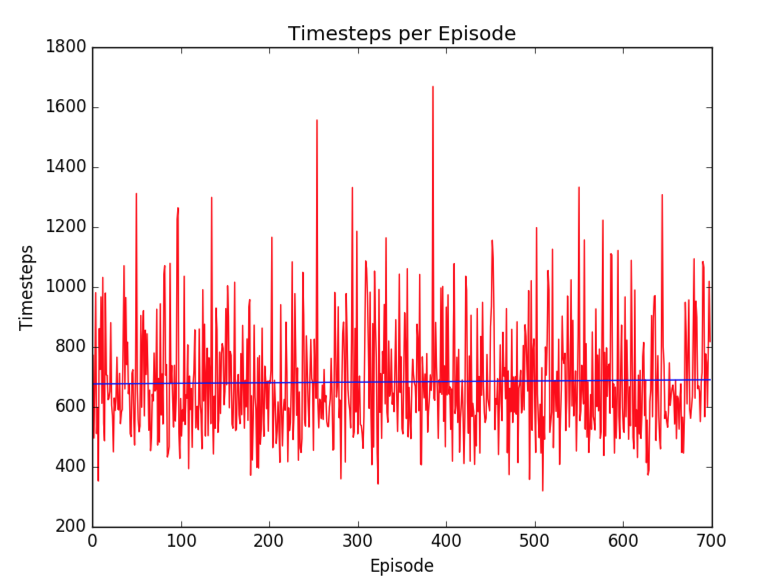
\includegraphics[scale=0.20]{timesteps_random}
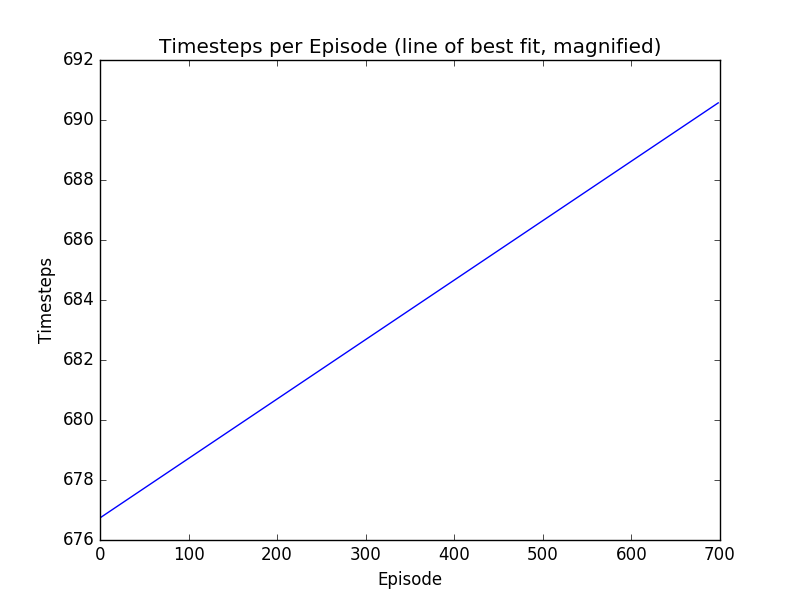
\includegraphics[scale=0.275]{timesteps_random_line_of_best_fit}
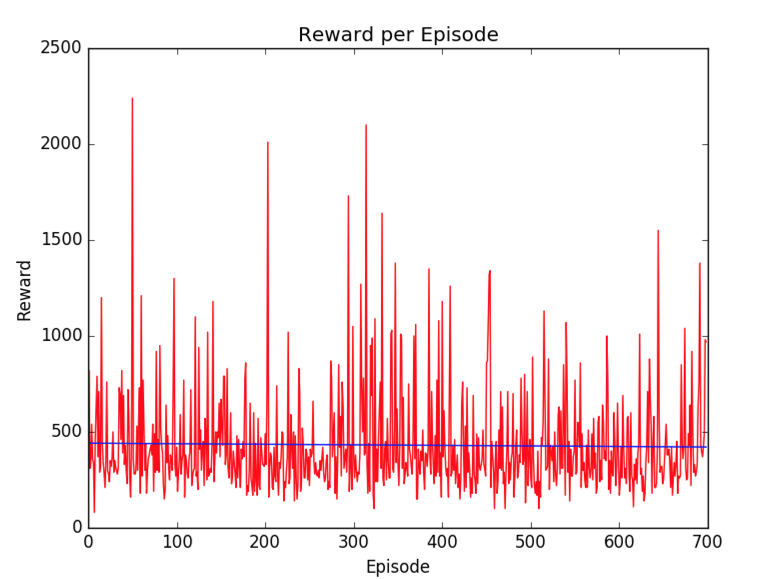
\includegraphics[scale=0.20]{reward_random}
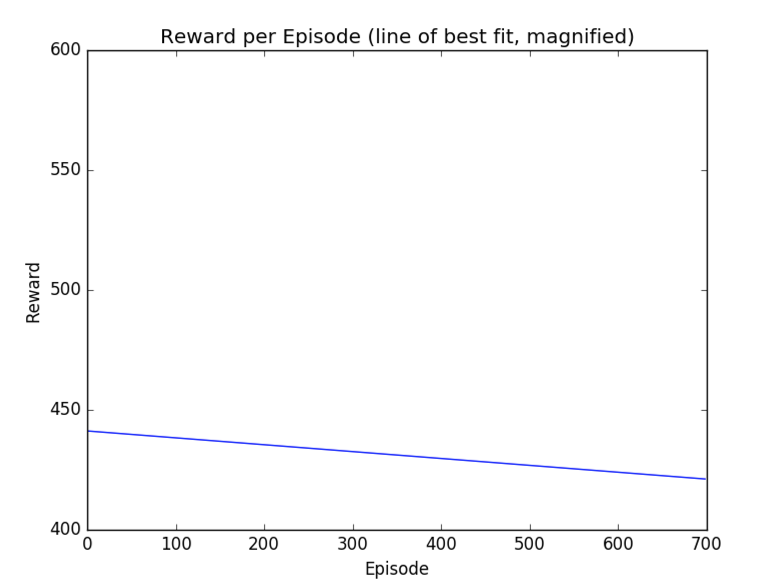
\includegraphics[scale=0.20]{reward_random_line_of_best_fit}
\centering
\caption{Random Agent Results}
\end{figure}

\begin{figure}[h]
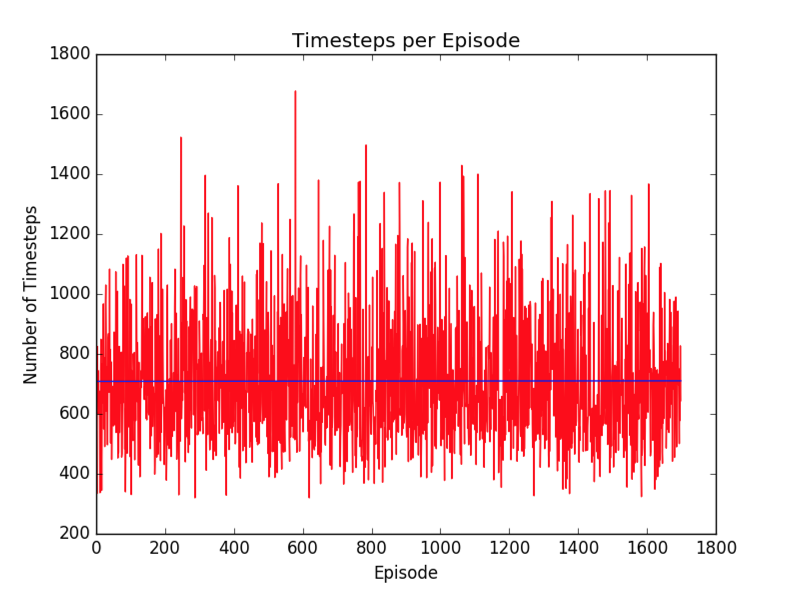
\includegraphics[scale=0.275]{timesteps_learned}
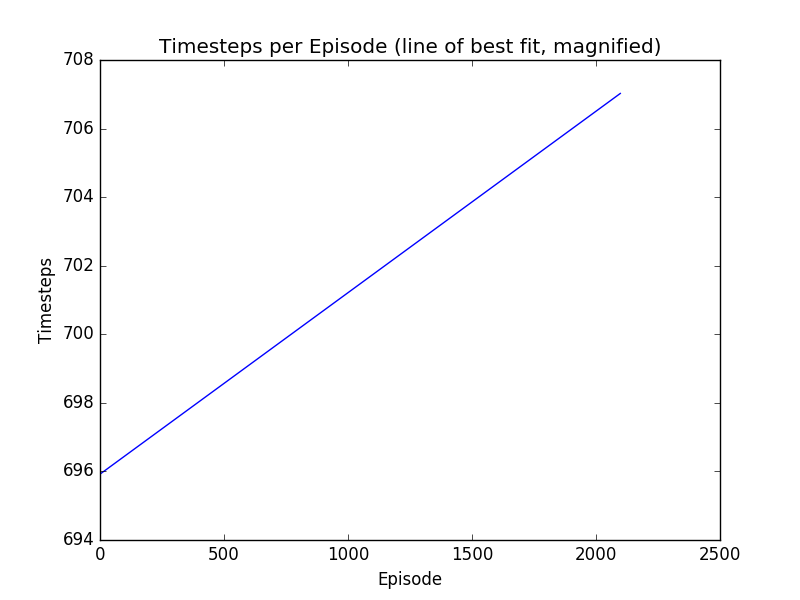
\includegraphics[scale=0.275]{timesteps_learned_line_of_best_fit}
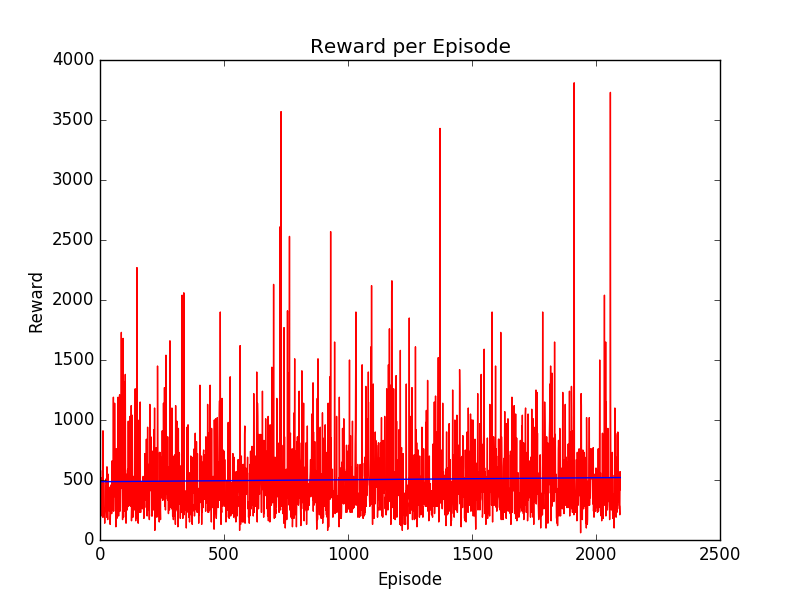
\includegraphics[scale=0.275]{reward_learned}
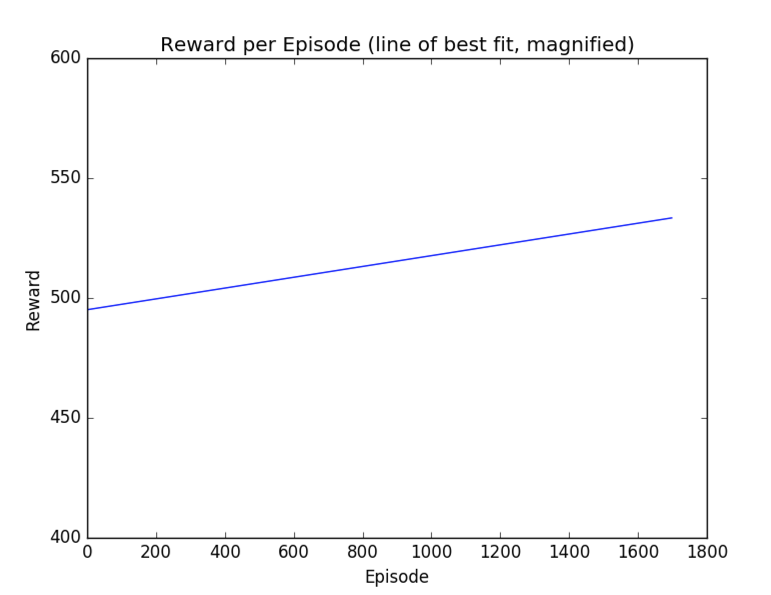
\includegraphics[scale=0.275]{reward_learned_line_of_best_fit}
\centering
\caption{Learning Agent Results}
\end{figure}




\section{Architectural Implementation Details}

We followed the implementation details proposed in the original (Mnih et. al., 2013) paper, with some minor hyperparameter modifications. The specifics of our implementation are provided below:

\begin{itemize}
\item \textbf{Data Preprocessing:} Before being passed into our network, each input frame is converted to grayscale and cropped to an 84x84 image. Four consecutive preprocessed images are stacked on top of each other to build a single representation of the game state which is subsequently passed into the network. An example of this process is provided in Figure 6.1.
\item \textbf{Deep Learning Architecture:} The implementation utilized in the paper has three hidden layers and one output layer. Utilizing the architectural description from the paper, ``The first hidden layer convolves 16 8x8 filters with stride 4 with the input image and applies a rectifier nonlinearity. The second hidden layer convolves 32 4x4 filters with stride 2, again followed by a rectifier nonlinearity. The final hidden layer is fully-connected and consists of 256 rectifier units. The output layer is a fully-connected linear layer with a single output for each valid action." It is important to note that, in the implementation utilized by the paper, the deep learning architecture actually simultaneously outputs Q-Values for every possible action the actor can take, given the input state. This differs slightly from the classical Q-Learning model, which generates Q-Values for (state, action) tuples.
\item \textbf{Loss:} \textit{Algorithm 1} in the original paper describes the details of the loss function utilized, which will be omitted here for brevity. However, it is important to note that this loss function is applied only to the output of the \textit{taken action}, an important caveat which caused us some difficulty. In our multi-output Q-Network, this implies that the ground-truth for non-taken actions utilized during backpropagation is actually the predicted value itself, making the loss zero and preventing the backpropagation of any error.
\item \textbf{Hyperparameters:} We utilized an epsilon value which started at 1.0 and decreased to a final value of 0.1 uniformly over a period of 100000 frames. Our experience replay capacity was set to 1000000, we utilized a minibatch size of 32, and a learning rate of 0.1. The original paper describes a frame-skipping process to increase the number of games played by the agent; we implemented this feature and set our frame-skip parameter to 4 (the value used in the paper).
\end{itemize}

\begin{figure}[h]
\includegraphics[scale=0.275]{game_state}
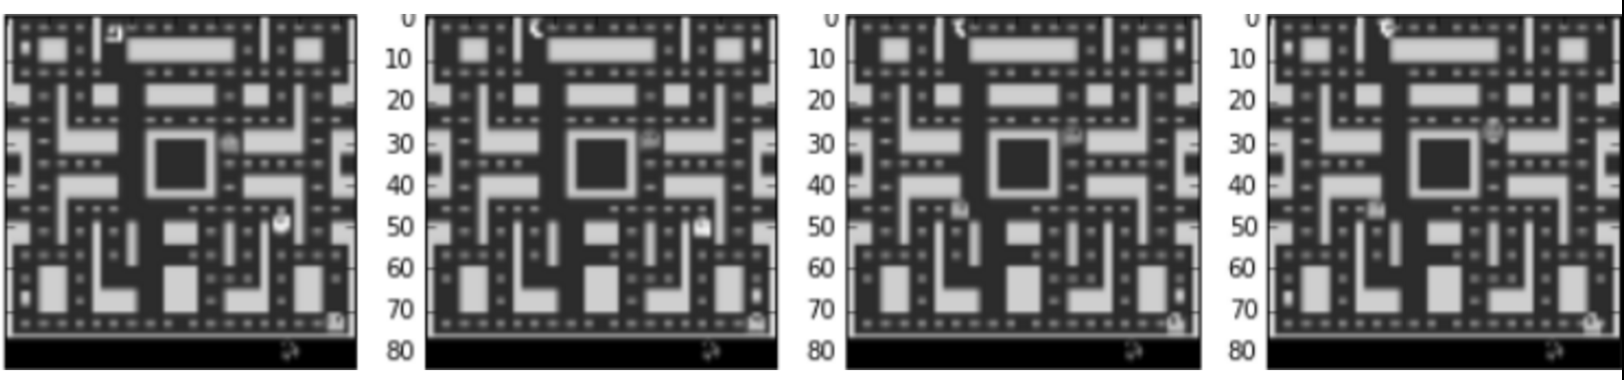
\includegraphics[scale=0.275]{preprocessed_game_state}
\centering
\caption{Example of our network input (before and after preprocessing)}
\end{figure}

\section{Miscellaneous Observations}

In future deep learning projects, we highly recommend the utilization of the OpenAI gym. The interface is clean and easy to use, and it includes many diverse reinforcement learning problems which would make for very interesting projects. In our case, it simplified emulator setup dramatically.

\section{Conclusion}

In our project, we implemented the core ideas proposed in the ``Playing Atari with Deep Reinforcement Learning" paper, and saw that our learner performs better than a random baseline. This result in and of itself is significant: given nothing but the input pixels from the screen, we have constructed a reinforcement learning agent which can learn something about playing Ms. Pac-Man. However, in our current results, our agent still performs worse than a human would. We propose that, with continued work on hyperparameter tuning and the utilization of longer training times on gpu-equipped machines, we should continue to see improvement in our agent's decision-making policy, with the hope that our implementation may eventually perform as well as humans. \\

We would allow our final writeup to appear on the course website.

\end{document}%%%%%%%%%%%%%%%%%%%%%%%%%%%%%%%%%%%%%%%%%



